\documentclass{beamer}
\mode<presentation>
\usepackage{amsmath}
\usepackage{amssymb}
%\usepackage{advdate}
\usepackage{graphicx}
\graphicspath{{../Figs/}}
\usepackage{adjustbox}
\usepackage{subcaption}
\usepackage{enumitem}
\usepackage{multicol}
\usepackage{mathtools}
\usepackage{listings}
\usepackage{url}
\def\UrlBreaks{\do\/\do-}
\usetheme{Boadilla}
\usecolortheme{lily}
\setbeamertemplate{footline}
{
  \leavevmode%
  \hbox{%
  \begin{beamercolorbox}[wd=\paperwidth,ht=2.25ex,dp=1ex,right]{author in head/foot}%
    \insertframenumber{} / \inserttotalframenumber\hspace*{2ex} 
  \end{beamercolorbox}}%
  \vskip0pt%
}
\setbeamertemplate{navigation symbols}{}

\providecommand{\nCr}[2]{\,^{#1}C_{#2}} % nCr
\providecommand{\nPr}[2]{\,^{#1}P_{#2}} % nPr
\providecommand{\mbf}{\mathbf}
\providecommand{\pr}[1]{\ensuremath{\Pr\left(#1\right)}}
\providecommand{\qfunc}[1]{\ensuremath{Q\left(#1\right)}}
\providecommand{\sbrak}[1]{\ensuremath{{}\left[#1\right]}}
\providecommand{\lsbrak}[1]{\ensuremath{{}\left[#1\right.}}
\providecommand{\rsbrak}[1]{\ensuremath{{}\left.#1\right]}}
\providecommand{\brak}[1]{\ensuremath{\left(#1\right)}}
\providecommand{\lbrak}[1]{\ensuremath{\left(#1\right.}}
\providecommand{\rbrak}[1]{\ensuremath{\left.#1\right)}}
\providecommand{\cbrak}[1]{\ensuremath{\left\{#1\right\}}}
\providecommand{\lcbrak}[1]{\ensuremath{\left\{#1\right.}}
\providecommand{\rcbrak}[1]{\ensuremath{\left.#1\right\}}}
\theoremstyle{remark}
\newtheorem{rem}{Remark}
\newcommand{\sgn}{\mathop{\mathrm{sgn}}}
\providecommand{\abs}[1]{\left\vert#1\right\vert}
\providecommand{\res}[1]{\Res\displaylimits_{#1}} 
\providecommand{\norm}[1]{\lVert#1\rVert}
\providecommand{\mtx}[1]{\mathbf{#1}}
\providecommand{\mean}[1]{E\left[ #1 \right]}
\providecommand{\fourier}{\overset{\mathcal{F}}{ \rightleftharpoons}}
%\providecommand{\hilbert}{\overset{\mathcal{H}}{ \rightleftharpoons}}
\providecommand{\system}[1]{\overset{\mathcal{#1}}{ \longleftrightarrow}}
%\providecommand{\system}{\overset{\mathcal{H}}{ \longleftrightarrow}}
	%\newcommand{\solution}[2]{\textbf{Solution:}{#1}}
%\newcommand{\solution}{\noindent \textbf{Solution: }}
\providecommand{\dec}[2]{\ensuremath{\overset{#1}{\underset{#2}{\gtrless}}}}
\newcommand{\myvec}[1]{\ensuremath{\begin{pmatrix}#1\end{pmatrix}}}
\let\vec\mathbf

\lstset{
%language=C,
frame=single, 
breaklines=true,
columns=fullflexible
}

\numberwithin{equation}{section}

\begin{document}


\title{4.3.58}
\author{AI25BTECH11002 - Ayush Sunil Labhade}
{\let\newpage\relax\maketitle}

\textbf{Question}:
		Show that the lines
		\begin{align}
\frac{x+3}{-3}=\frac{y-1}{1}=\frac{z-5}{5}
		\end{align}
		\begin{align}
		\frac{x+1}{-1}=\frac{y-2}{2}=\frac{z-5}{5}
		\end{align}
are coplanar.
	


\textbf{Solution:}

The given lines are
\begin{align}
L_1 &: \frac{x+3}{-3}=\frac{y-1}{1}=\frac{z-5}{5} \\
L_2 &: \frac{x+1}{-1}=\frac{y-2}{2}=\frac{z-5}{5}
\end{align}

In vector form:
\begin{align}
\vec{L_1} &= \myvec{-3 \\ 1 \\ 5}\lambda + \myvec{-3 \\ 1 \\ 5} \\
\vec{L_2} &= \myvec{-1 \\ 2 \\ 5}\mu + \myvec{-1 \\ 2 \\ 5}
\end{align}

So the direction vectors are
\begin{align}
	\vec{m_1} &= \myvec{-3 \\ 1 \\ 5} \quad 
	\vec{m_2} &= \myvec{-1 \\ 2 \\ 5}
\end{align}
and the vector between points on the two lines is
\begin{align}
\vec{B}-\vec{A} = \myvec{-1 \\ 2 \\ 5} - \myvec{-3 \\ 1 \\ 5} = \myvec{2 \\ 1 \\ 0}
\end{align}

For coplanarity, we check
\begin{align}
rank \myvec{ \vec{m_1} & \vec{m_2} & \vec{B}-\vec{A} } \leq 2
\end{align}

That is,
\begin{align}
	\vec{M} = \myvec{ 
-3 & -1 & 2 \\
1 & 2 & 1 \\
5 & 5 & 0 
}.
\end{align}

Perform row reduction:

\begin{align}
\myvec{
-3 & -1 & 2 \\
1 & 2 & 1 \\
5 & 5 & 0
}
\xrightarrow[]{R_1 \leftrightarrow R_2}
\myvec{
1 & 2 & 1 \\
-3 & -1 & 2 \\
5 & 5 & 0
}
\end{align}

\begin{align}
\xrightarrow[]{R_2 \to R_2 + 3R_1,\; R_3 \to R_3 - 5R_1}
\myvec{
1 & 2 & 1 \\
0 & 5 & 5 \\
0 & -5 & -5
}
\end{align}

\begin{align}
\xrightarrow[]{R_3 \to R_3 + R_2}
\myvec{
1 & 2 & 1 \\
0 & 5 & 5 \\
0 & 0 & 0
}
\end{align}

Now the matrix is in echelon form.  

The rank of the matrix is \(2\).

$\therefore$ the given lines are coplanar.
		

Graph:
\begin{figure}[H]
    \centering
    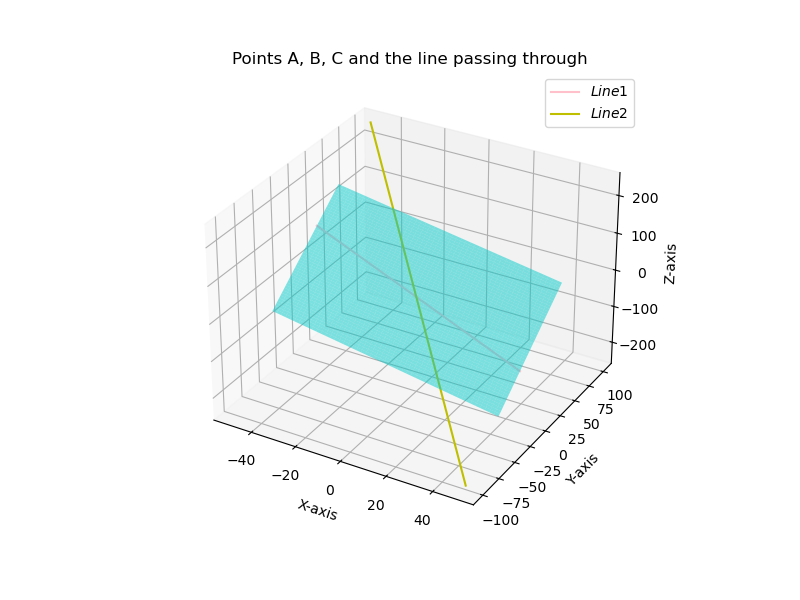
\includegraphics[scale=0.5]{plot}
    \caption{}
    \label{fig:plot}
\end{figure}
\end{document}
